% $Id: INF_Poster_example.tex 7714 2011-08-31 17:34:46Z tkren $
%
% TU Wien - Faculty of Informatics
% poster template
%
% This template is using the beamer document class and beamerposter package, see
% <http://www.ctan.org/tex-archive/macros/latex/contrib/beamer/>
% <http://www.ctan.org/tex-archive/macros/latex/contrib/beamerposter/>
% <http://www-i6.informatik.rwth-aachen.de/~dreuw/latexbeamerposter.php>
%
% For questions and comments send an email to
% Thomas Krennwallner <tkren@kr.tuwien.ac.at>
%

\documentclass[final,hyperref={pdfpagelabels=true}]{beamer}

\usepackage{TUINFPST}
\usepackage{graphicx}
\usepackage{lipsum}
\usepackage{subfig}
\usepackage{caption}
\usepackage{wrapfig}
 
%\title[Computational Intelligence]{Interactive Computer Generated Architecture}
% if you have a long title looking squeezed on the poster, just force
% some distance:
\title[Computational Intelligence]{%
  Meta-Heuristic Local Planning \\[0.2\baselineskip]%
  %Description Logics into HEX-Programs %\\[0.2\baselineskip]%
}
\author[markus.suchi@tuwien.ac.at]{Markus Suchi}
\institute[]{%
  Technische Universit{\"a}t Wien\\[0.25\baselineskip]
  Institut f{\"u}r Automatisierungs- und Regelungstechnik\\[0.25\baselineskip]
  %Arbeitsbereich: Vision for Robotics\\[0.25\baselineskip]
  Betreuer: Ao.Univ.-Prof. Dipl.-Ing. Dr. Markus Vincze
}
%\titlegraphic{\includegraphics[height=52mm]{logo_KBS_2_CMYK}}
\titlegraphic{\includegraphics[height=52mm]{nologo}}
\date[\today]{\today}
\subject{epilog}
\keywords{my kwd1, my kwd2}

%%%%%%%%%%%%%%%%%%%%%%%%%%%%%%%%%%%%%%%%%%%%%%%%%%%%%%%%%%%%%%%%%%%%%%%%%%%%%%%%%%%%%%

% Display a grid to help align images 
%\beamertemplategridbackground[12.7mm]

% play around with the background colors
% \setbeamercolor{background canvas}{bg=yellow}

% use a background picture
% \usebackgroundtemplate{%
%   \includegraphics[width=\paperwidth]{logo_KBS_2_CMYK}
% }

% play around with block colors
\setbeamercolor{block body}{fg=black,bg=white}
\setbeamercolor{block title}{fg=TuWienBlue,bg=white}

\setbeamertemplate{block begin}{
  \begin{beamercolorbox}{block title}%
    
\begin{tikzpicture}%
      \node[draw,rectangle,line width=3pt,rounded corners=0pt,inner sep=0pt]{%
        \begin{minipage}[c][2cm]{\linewidth}
          \centering\textbf{\insertblocktitle}
        \end{minipage}
      };
    \end{tikzpicture}%
  \end{beamercolorbox}
  \vspace*{1cm}
  \begin{beamercolorbox}{block body}%
}

\setbeamertemplate{block end}{
  \end{beamercolorbox}
  \vspace{2cm}
}

% setup postit
\setbeamercolor{postit}{fg=black,bg=yellow} 
\newenvironment{postit}
{\begin{beamercolorbox}[sep=1em,wd=7cm]{postit}}
{\end{beamercolorbox}}


% for crop marks, uncomment the following line
%\usepackage[cross,width=88truecm,height=123truecm,center]{crop}

%%%%%%%%%%%%%%%%%%%%%%%%%%%%%%%%%%%%%%%%%%%%%%%%%%%%%%%%%%%%%%%%%%%%%%%%%%%%%%%%%%%%%%

\begin{document}

% We have a single poster frame.
\begin{frame}
  \begin{columns}[t]
    % ---------------------------------------------------------%
    % Set up a column
    \begin{column}{.45\textwidth}
      \begin{block}{Motivation}

        Navigation is a vital task for mobile robots driving through dynamic environments. 
        A common approach divides this task into two parts:
        \begin{itemize}
        \item global planning creates a path from start to goal to guide the robot
        \item local planning uses obstacle avoidance methods to safely follow the guide
        \end{itemize}
       	\begin{figure}
       	 \captionsetup[subfigure]{labelformat=empty} 
         \subfloat[Global and local planning]
         {  
           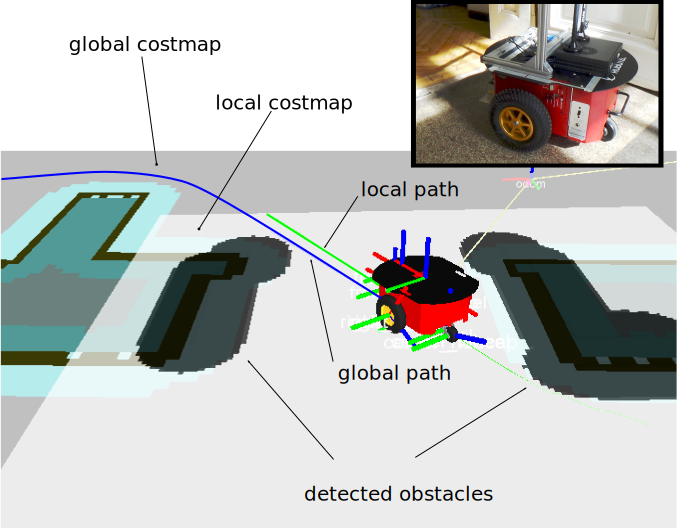
\includegraphics[width=0.50\textwidth]{pioneer.jpeg}
         }
         \subfloat[Trajectory selection in local planning]
         {  
           \includegraphics[width=0.39\textwidth]{fig_inst_25_new_cmyk.jpeg}
         }      
       \end{figure}        
       
        Very effective local planning methods like the Dynamic Window Approach \cite{DWA1997} are based on sampling the 2-dim velocity space of the robot vehicle.
        Possible linear and angular velocities $(v,w)$ are used as control values and their application is simulated for a short period of time. 
        
        The resulting trajectories are weighted using a costfunction.
        The velocity tuple yielding the best trajectory is then propagated to the motor controller of the robot.     
        
        The goal of this work is to analyze these local planning approaches and improve the selection process by using meta-heurstics. 
  \end{block}
  
            \begin{block}{Approach}
      Well known meta-heuristic algorithms are used to speed up the local planning within the trajectory selection step.
      For this purpose the velocity space is structured according to the following neighborhood definition:
\begin{itemize}
 \item $N_0(x)=$ 4-connected
 \item $N_1(x)=$ 8-connected
 \item $\dots$
 \item $N_k(x)=$ k-steps reachable neighborhood.
\end{itemize}
       \begin{figure}
          \includegraphics[width=0.60\columnwidth]{fig_neighborhood3d_cmyk.jpeg}     
       \end{figure}

      These neighborhoods are used by the following meta-heuristic algorithms: 
      \begin{itemize}
        \item Random Search with Tabu List (Random)
 		\item Iterated Local Search with fixed sized neighborhoods (ILS4,ILS8,ILS16)
 		\item Variable Neighborhood Search with Best-, and First-Improvement heuristic (VNSF,VNSB)
       \end{itemize}
        \end{block}  
                     
    \end{column}
    % ---------------------------------------------------------%
    % end the column

    % ---------------------------------------------------------%
    % Set up a column 
    \begin{column}{.45\textwidth}             
      \begin{block}{Step 1: Evaluation on static obstacle maps}
       The algorithms were tested on 60 randomly generated static obstacle maps and a simple local planning component.
       Results are documenting a significant performance increase:
       \begin{figure}
                %\centering
    			%\myfloatalign
                 %\setlength\fboxsep{0pt}
                 %\setlength\fboxrule{0.5pt}
         \captionsetup[subfigure]{labelformat=empty} 
         \subfloat[240 trajectories]
         {  
           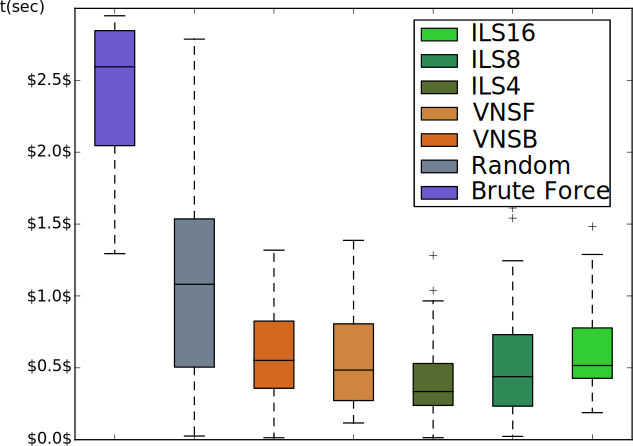
\includegraphics[width=0.45\textwidth]{fig_allworlds_6_40.jpeg}
         }
         \subfloat[2400 trajectories]
         {  
           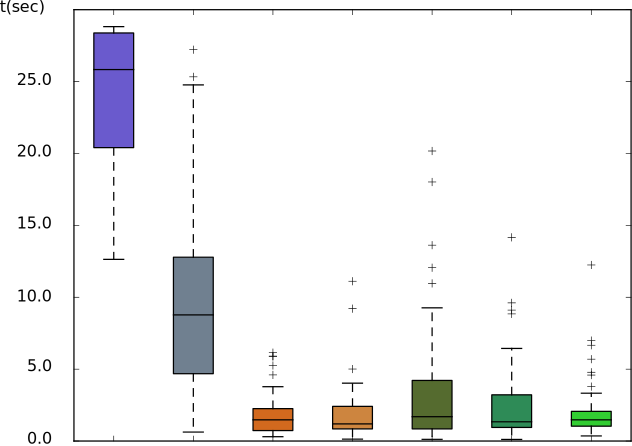
\includegraphics[width=0.45\textwidth]{fig_allworlds_24_100.jpeg}
         }\\
         \subfloat[]
         {  
           
\includegraphics[width=0.6\textwidth]{legend_all.jpeg}
         }                
       \end{figure}
      \end{block}

      \begin{block}{Step 2: Integration into existing planning systems}
        The VNS approach was selected to be integrated into a state of the art planning system for mobile robots based on Trajectory Rollout (VNS-ROL) and DWA ((VNS-DWA) \cite{DBLP:conf/icra/Marder-EppsteinBFGK10}. The different planners are tested in two virtual environments using a 3D-physics simulation.
       \begin{figure}
                %\centering
    			%\myfloatalign
                 %\setlength\fboxsep{0pt}
                 %\setlength\fboxrule{0.5pt}
         \captionsetup[subfigure]{labelformat=empty} 
         \subfloat[3D-Model]
         {  
           \includegraphics[width=0.5\textwidth]{fig_gh25_gazebo_cmyk.jpeg}
         }
         \subfloat[View of the robot]
         {  
           \includegraphics[width=0.5\textwidth]{fig_gh25_rviz_cmyk.jpeg}
         }                
       \end{figure}
       
       The results show, that the VNS approach outperform the brute-force method of the original implementations.
       
        \begin{figure}
                %\centering
    			%\myfloatalign
                 %\setlength\fboxsep{0pt}
                 %\setlength\fboxrule{0.5pt}
         \captionsetup[subfigure]{labelformat=empty} 
         \subfloat[]
         {  
           \includegraphics[width=0.95\textwidth]{fig_logo_rol_dwa.jpeg}
         }\\
         \subfloat[]
         {  
           
\includegraphics[width=0.4\textwidth]{legend_rol.jpeg}
         }\hspace{30mm}      
         \subfloat[]
         {  
           \includegraphics[width=0.4\textwidth]{legend_dwa.jpeg}
         }            
       \end{figure}
      \end{block}
	  
      \begin{block}{References}
        \small
        \bibliographystyle{plain}
	    \bibliography{Bibliography}
	  \end{block}

    \end{column}
    % ---------------------------------------------------------%
    % end the column
  \end{columns}

%  \begin{tikzpicture}[remember picture,overlay]
%    \node[inner sep=0pt,xshift=-30cm,yshift=23cm] at (current page.east) {%
%      \begin{postit}%
%        Post-It time!%
%      \end{postit}%
%    }; 
%  \end{tikzpicture}
  %\begin{columns}[t]
    % ---------------------------------------------------------%
    % Set up a column
    %\begin{column}{\textwidth}
        
%        \begin{thebibliography}{999}
%          
%        \bibitem[Foo~and~Fu, 2010]{ff2010}
%          Foo, B.; and Fu, B.
%          2010.
%          {On logical representations of hackerisms}.
%          {\em J.~Log.~Hack.} 1:1--2.
%          
%        \bibitem[Crock~et~al., 2010]{ck2010}
%          Crock, A; Cruft, B.; and Kludge, C.
%          2010.
%          {Decomposing junk code}.
%          Manuscript.
%          
%        \end{thebibliography}
    %\end{column}
   %\end{columns}
   
\end{frame}


   
\end{document}

%%% Local Variables:
%%% TeX-PDF-mode: t
%%% TeX-debug-bad-boxes: t
%%% TeX-master: t
%%% TeX-parse-self: t
%%% TeX-auto-save: t
%%% reftex-plug-into-AUCTeX: t
%%% End:
